
El objeto principal de estudio de este trabajo es el mu\'on, que se trata de una part\'icula elemental cargada con spin 1/2 y con masa aproximadamente 200 veces mayor que el electr\'on, siendo adem\'as una part\'icula inestable con un tiempo de vida de 2.2 $\mu s$, que es elevado en comparaci\'on con otras part\'iculas que poseen esta caracter\'istica. \\

En este trabajo nos centraremos espec\'ficamente en la detecci\'on y reconstrucci\'on de muones en el detector CMS (del ingl\'es \textit{Compact Muon Solenoid}), situado en el gran colisionador de hadrones LHC (del ingl\'es \textit{Large Hadron Collider}). La mayor parte de los muones medidos por CMS provienen t\'ipicamente de desintegraciones de quarks top, de hadrones o de desintegraciones lept\'onicas de bosones $Z$ o $W$~\cite{PhysRevD.98.030001}. Estos muones se caracterizan normalmente por tener un momento transverso o $p_{T}$ inferior a 200 GeV y se categorizan como muones de bajo momento o \textit{low-$p_{T}$ muons}. \\
Por otra parte, los muones de alto momento o \textit{high-$p_{T}$ muons} pueden tener como origen procesos f\'isicos at\'ipicos como la desintegraci\'on de part\'iculas ex\'oticas fuera del Modelo Est\'andard de la f\'isica de part\'iculas~\cite{gaillard1999standard} como bosones $Z'$ o $W'$~\cite{CMS-PAS-EXO-19-019,2017278} con masas en la escala del TeV, cuyo descubrimiento ser\'ia un indicativo directo de nueva f\'sica, por lo que medir las propiedades de estos muones de la manera m\'as precisa posible en el detector es de vital importancia. Concretamente, el objetivo principal del trabajo es aplicar una t\'ecnica de regresi\'on basada en una red neuronal profunda o DNN (del ingl\'es \textit{Deep Neural Network})~\cite{Schmidhuber:2015} para estimar el momento transverso de los \textit{high-$p_{T}$ muons} con precisi\'on. \\

Experimentalmente, la medida del momento de los \textit{high-$p_{T}$ muons} plantea varias dificultades. Primero, hay que tener en cuenta que la resoluci\'on de la medida de $p_{T}$ a partir de la traza empeora cuando el momento del mu\'on aumenta. \\
En presencia de un campo magn\'etico uniforme $B$, y con un radio de curvatura de la traza $R$, el momento transverso $p_{T}$ de un mu\'on con carga $q$ se puede expresar a trav\'es de la ecuaci\'on de Lorentz como:

\begin{equation}
  p_{T}[\text{GeV}] = 0.3 \times B[\text{T}] \times R[\text{m}] \times q
\label{eq:pTvsRadius}
\end{equation}

El campo campo magn\'etico dentro del solenoide de CMS es pr\'acticamente uniforme y conocido con gran precisi\'on ($B$ = 3.8 T), mientras que el radio de curvatura se relaciona con la longitud del arco $L$ y la distancia sagitta $s$ definida en la Figura~\ref{fig:SagittaDef} a trav\'es de:

\begin{equation}
  R[\text{m}]\approx L[\text{m}]^{2}/8s[\text{m}]
\label{eq:RadiusvsSagitta}
\end{equation}

Esta aproximaci\'on es v\'alida para $L/R \ll 1$. \\

Combinando las ecuaciones \eqref{eq:pTvsRadius} y \eqref{eq:RadiusvsSagitta} se obtiene:

\begin{equation}
  s[\text{m}]\approx (0.3 B [\text{T}] L[\text{m}]^{2}/8) (q/p_{T}[\text{GeV}]) =  (0.3 BL^{2}/8) \times (q/p_{T}),
\label{eq:SagittavsPt}
\end{equation}

Se observa que $s$ es inversamente proporcional al momento transverso, por lo que para mejorar la resoluci\'on en la medida del $p_{T}$ en los casos con sagittas peque\~nas, las trazas de los muones en CMS se reconstruyen en distintos subdetectores separados a varios metros del punto de colisi\'on, como se detallar\'a en la Secci\'on~\ref{sec:CMS}, para as\'i tener trazas de mayor longitud y por consiguiente mayores valores de $s$. Hay que tener en cuenta que medir $s$ con precisi\'on puede ser un gran desaf\'io; por ejemplo un mu\'on con $p_{T}$= 200 GeV que atraviesa CMS presenta un valor de sagitta del orden del mil\'imetro.  \\
Sin embargo, aunque esto mejora considerablemente la resoluci\'on en la medida de $p_{T}$, sagitta sigue siendo peque\~na para muones de muy alto momento en la escala del TeV, y adem\'as la medida de $s$ se puede ver afectada por fallos en el alineamiento de las se\~nales que componen la traza. \\

\begin{figure}[h]
\centering
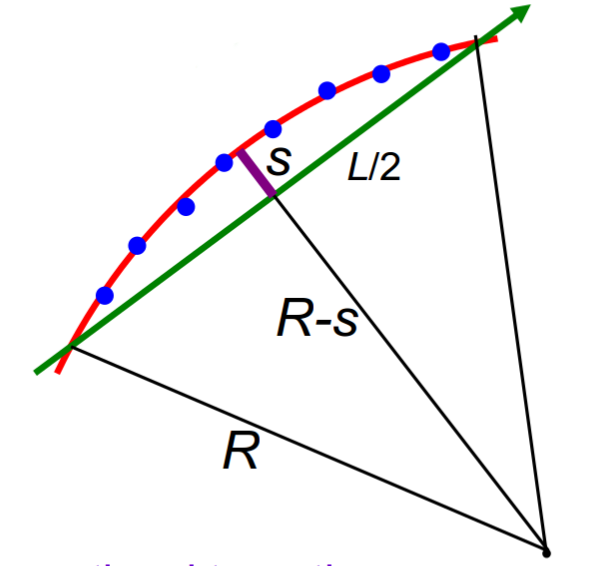
\includegraphics[width=0.30\textwidth]{figures/curvaturesketch.png}
\caption{Definici\'on de la distancia saggita, $s$, a partir de la longitud de la traza reconstruida $L$ y de su radio $R$.}
\label{fig:SagittaDef}
\end{figure}

Por otra parte, cuando los muones de alto momento atraviesan el hierro, las p\'erdidas de energ\'ia por radiaci\'on tales como producci\'on de pares, Bremsstrahlung, o interacciones fotonucleares no son despreciables comparadas con la p\'erdida de energ\'ia por ionizaci\'on. En la Figura~\ref{fig:dEdX} se muestra la dependencia de la p\'erdida de energ\'ia del mu\'on por unidad de distancia $dE/dx$ al atravesar distintos medios como funci\'on de su energ\'ia.

\begin{figure}
\centering
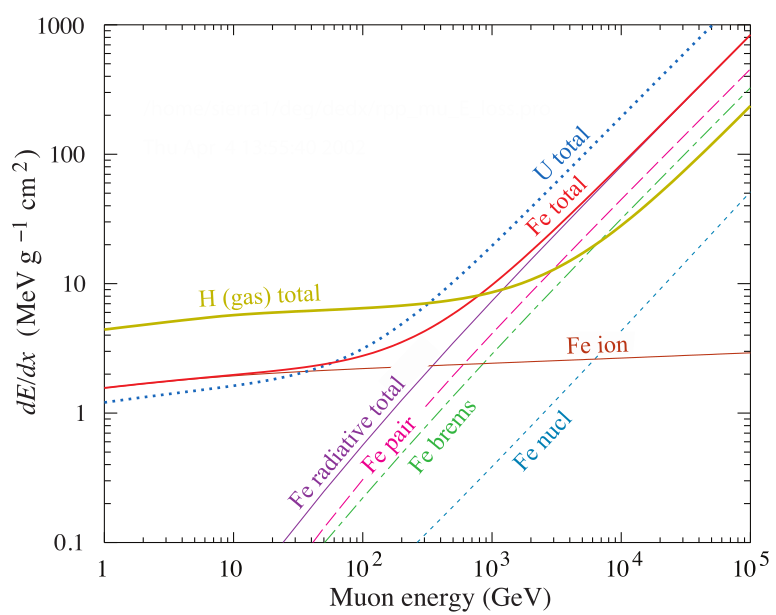
\includegraphics[width=0.60\textwidth]{figures/dEdx.png}
\caption{Media de la p\'erdida de energ\'ia por ionizaci\'on y por radiaci\'on de un mu\'on en hidr\'ogeno, hierro y uranio como funci\'on de su energ\'ia.  Average energy loss from ionization and radiative loss of a muon in hydrogen, iron and uranium as a function of its energy. En el caso del hierro, se separan las contribuciones a $dE/dx$ para producci\'on de pares, Bremsstrahlung e interacciones fotonucleares. Figura tomada de \cite{Tanabashi:2018oca}.}
\label{fig:dEdX}        
\end{figure}

Se observa que la energ\'ia cr\'itica para el hierro, $E^{iron}_{c}$, donde la energ\'ia de ionizaci\'on (en marr\'on) es igual a la suma de todas las p\'erdidas radiativas (en morado) ocurre aproximadamente a 300 GeV. Como consecuencia, la principal fuente de p\'erdida de energ\'ia para un mu\'on con $E>E^{iron}_{c}$ que viaja por hierro a trav\'es de los distintos subdetectores de CMS es debida a radiaci\'on electromagn\'etica fruto de la producci\'on de electrones y fotones. \\
Esta radiaci\'on electromagn\'etica se manifiesta en el detector como una cascada de part\'iculas (\textit{muon shower}) que producen se\~nales adicionales en los detectores, y puede incluso cambiar la direcci\'on de la trayectoria del mu\'on, afectando negativamente a la reconstrucci\'on de su traza y degradando por consiguiente la medida de su momento. \\

Los algoritmos de reconstrucci\'on de trazas que son utilizados para la asignaci\'on del momento transverso a los muones \textit{high-$p_{T}$} en CMS evitan lidiar con casos de emisi\'on de cascadas, como se explicar\'a con m\'as detalle en la Secci\'on~\ref{sec:current_assignment}. De esta manera, por ejemplo, si se encuentran varios impactos en un subdetector que puedan ser indicativo de que una cascada ha tenido lugar, t\'ipicamente se ignoran estas se\~nales a la hora de reconstruir la traza del mu\'on. \\
El objetivo de este trabajo, por contrapartida, es recopilar toda la informaci\'on posible de la trayectoria de los muones a su paso por CMS (incluyendo los impactos provenientes de cascadas electromagn\'eticas) utilizando para ello muones simulados altamente energ\'eticos con $p_{T}$ generado conocido (el momento real asignado en la simulaci\'on de la partícula), y entrenar posteriormente una DNN que haga regresi\'on al $p_{T}$ reconstruido, de manera que se consiga una asignaci\'on de momento transverso mejor que el proporcionado por los algoritmos centrales de CMS. \\

Para cuantificar la calidad de la asignaci\'on del momento transverso, se har\'a uso de la resoluci\'on $R$, definida como:

\begin{equation}
  R = \dfrac{\lvert p_{T}^{GEN} - p_{T}^{RECO}\rvert}{p_{T}^{GEN}}
\label{eq:R}
\end{equation}

Donde $p_{T}^{GEN}$ hace referencia al momento generado del mu\'on y $p_{T}^{RECO}$ al momento reconstruido a trav\'es de su traza en el detector. \\

La presente memoria est\'a estructurada en las siguientes secciones. En la Secci\'on~\ref{sec:CMS} se describir\'a brevemente el dispositivo experimental utilizado: el detector CMS. Posteriormente, en la Secci\'on~\ref{sec:current_assignment} se presentar\'an los algoritmos actuales utilizados para la asignaci\'on de momento. En la Secci\'on~\ref{sec:methodology} se describir\'a el m\'etodo propuesto, es decir, c\'omo se realiza la selecci\'on de muones y hits sobre la muestra de simulaci\'on utilizada. En la Secci\'on~\ref{sec:training} se detallar\'a c\'omo se construyen las variables de entrenamiento, la arquitectura de la red utilizada, y los resultados del entrenamiento. Por \'ultimo, en las Secciones~\ref{sec:results} y \ref{sec:conclusions} se mostrar\'an los resultados finales y las conclusiones del trabajo.
